% $Header: /project/cl/Root/CVS/talks/iowa08/talk.tex,v 1.3 2008/01/31 14:11:37 stump Exp $

\documentclass[11pt]{beamer}

\usepackage{tikz}
\usepackage{pgflibraryarrows}
\usepackage{pgflibraryshapes}
\usepackage{pgfbaseimage}
\usepackage{proof}
\usepackage{url}

\newcommand{\Eq}[0]{\texttt{=}}
\newcommand{\Neq}[0]{\texttt{!=}}
\newcommand{\Qeq}[0]{\stackrel{?}{=}}
\newcommand{\bang}[0]{\texttt{!}}
\newcommand{\quant}[0]{\textit{Quant}}

\newcommand{\To}[0]{\Rightarrow}
\newcommand{\rn}[1]{\textsc{#1}}
\newcommand{\interp}[1]{[ \negthinspace [ #1 ] \negthinspace ]}

\newcommand{\seq}[3]{#1 \vdash #2 : #3}
%\newcommand{\aseq}[3]{ #2 : #3}
\newcommand{\aseq}[3]{ #1 \vdash #3}
%\newcommand{\aaseq}[3]{ #3}
\newcommand{\aaseq}[3]{ #1 \vdash #3}
\newcommand{\abseq}[3]{ #1 \vdash #3}


\mode<presentation>
{
  %\usetheme{Warsaw}
  % or ...

%\usetheme{IowaCity}
%\usetheme{Edinburgh}
\usetheme{Savannah}

%  \setbeamercovered{transparent}
  % or whatever (possibly just delete it)
}


\usepackage[english]{babel}
% or whatever

\usepackage[latin1]{inputenc}
% or whatever

\usepackage{times}
\usepackage[T1]{fontenc}
% Or whatever. Note that the encoding and the font should match. If T1
% does not look nice, try deleting the line with the fontenc.

\title[Verified Programming in Guru]
{Verified Programming in Gugu}

\author[Stump et al.]{Aaron Stump\inst{1} \and Morgan Deters\inst{2} \and Adam Petcher\inst{3} \and Todd~Schiller\inst{3} \and Timothy Simpson\inst{3}}

\institute[Computational Logic Center]
{
\inst{1}
  Computational Logic Center\\
  CS, The University of Iowa
\and
\inst{2} LSI, Universitat Polit\`{e}cnica de Catalunya, Spain
\and
\inst{3} CSE, Washington University in St. Louis

\ \\
\ \\
Funding from NSF CAREER. 
}

\pgfdeclareimage[height=2cm]{laundry}{laundry}
\pgfdeclareimage[height=3cm]{car}{repaired-car}

% If you have a file called "university-logo-filename.xxx", where xxx
% is a graphic format that can be processed by latex or pdflatex,
% resp., then you can add a logo as follows:

% \pgfdeclareimage[height=0.5cm]{university-logo}{university-logo-filename}
% \logo{\pgfuseimage{university-logo}}



% Delete this, if you do not want the table of contents to pop up at
% the beginning of each subsection:
%\AtBeginSubsection[]
%{
%  \begin{frame}<beamer>
%    \frametitle{Outline}
%    \tableofcontents[currentsection,currentsubsection]
%  \end{frame}
%}


% If you wish to uncover everything in a step-wise fashion, uncomment
% the following command: 

%\beamerdefaultoverlayspecification{<+->}

\begin{document}

\date{\ }

\begin{frame}[plain]
  \titlepage
\end{frame}

\date{PLPV '09}

\begin{frame}
  \frametitle{A Vexing Continuum}

\begin{center}

\begin{tikzpicture}
\draw (0,0) node[anchor=south west,text=red] {Real code} -- (10,0) node[anchor=south east,text=red] {Math. functions};
\end{tikzpicture}

 \ \ \ \ 
\begin{tabular}{l}
concurrent \\
imperative \\
general recursive
\end{tabular}
\ \ \ \ \ \ \ \ \ \ \ \ \ \ \ \ \ \ \ \ \ \ \ \ \ \ \ \ \ \ \ \ \ \ \ \ \ \ \ \ 
\begin{tabular}{l}
sequential \\
pure \\
terminating
\end{tabular}
\ \ 

\ 

\ 

\ 

Where is your verification method?

\end{center}

\end{frame}

\begin{frame}
  \frametitle{Plotting Some Approaches}

\begin{center}
\begin{tikzpicture}
\draw (0,5) -- (0,2.5) node[anchor=east,text=blue] {\begin{tabular}{l}Verification\\ power\end{tabular}} -- (0,0) node[anchor=north,text=red] {Real code} -- (8,0) node[anchor=north,text=red] {Math};

\fill (0,1) circle (2pt) node[right=2pt] {\small Model Checking} ;

\fill (1,2) circle (2pt) node[right=2pt] {\small Static Analysis} ;

\fill (4,3.5) circle (2pt) node[right=2pt] {\small Dependently Typed PL};

\fill (8,5) circle (2pt) node[above=2pt] {\small Type Theory};

\end{tikzpicture}

\end{center}

\end{frame}

\begin{frame}
  \frametitle{The \textsc{Guru} Approach}

\begin{center}
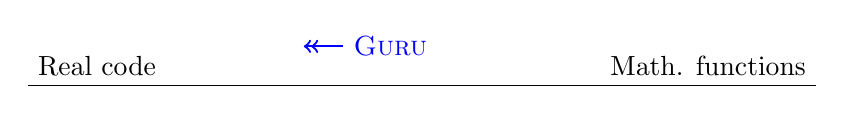
\begin{tikzpicture}
\draw (0,0) node[anchor=south west] {Real code} -- (10,0) node[anchor=south east] {Math. functions};
\draw[thick,->>,color=blue] (4,0.5) node[anchor=west,text=blue] {\textsc{Guru}} -- (3.5,0.5) ;
\end{tikzpicture}

\ 

\ \ \ \ \ \ \ \ \ \ \ \ \ \ \ \ \ \ \ 
\begin{tabular}{l}
\textcolor{blue}{General recursion} \\
\textcolor{blue}{Dependently typed programs} \\
\textcolor{blue}{External theorems about programs }\\
\textcolor{blue}{Mutable state} \\
No concurrency \\ 
No aliasing (yet)
\end{tabular}

\end{center}

\end{frame}

\begin{frame}
  \frametitle{Basic \textsc{Guru} Design}

\begin{itemize}

\item Terms : Types.
\item Proofs : Formulas.
\item ``Full-spectrum'' dependency.
\item Proofs and types can appear in terms.
\begin{itemize}
\item computationally irrelevant.
\item erased by compilation, definitional equality.
\end{itemize}

\item Definitional equality is very weak (no $\beta$).

\item Type checking decidable.

\item Explicit casts.

\ 

\item \textcolor{blue}{Today:} 
\begin{itemize}

\item specificational data.
\item ownership annotations.
\item functional modeling.

\end{itemize}

\end{itemize}


\end{frame}

\begin{frame}
  \frametitle{Specificational Data}

\begin{itemize}

\item Programmer can designate argument positions \texttt{spec}.

\begin{itemize}
\item for constructors, functions.
\item \texttt{spec} \texttt{x} can only be used in a \texttt{spec} position.
\item enforced separately from type checking.
\end{itemize}

\item \texttt{spec} args erased by compilation \textcolor{purple}{[Brady+03]}, def. equality.

\item Improves efficiency, simplifies proofs.

\end{itemize}
\end{frame}

\begin{frame}[containsverbatim]
\frametitle{Example: Vector Append}
\footnotesize
\begin{verbatim}
Inductive vec : Fun(A:type)(n:nat).type :=
  vecn : Fun(A:type).<vec A Z>
| vecc : Fun(A:type)(spec n:nat)(a:A)(l:<vec A n>).
              <vec A (S n)>.

vec_append : Fun(A:type)(spec n m:nat)
                (l1 : <vec A n>)(l2 : <vec A m>).
                <vec A (plus n m)>

vec_append_assoc : 
  Forall(A:type)(n1 : nat)(l1 : <vec A n1>)
        (n2 n3 : nat)(l2 : <vec A n2>)(l3 : <vec A n3>).
  { (vec_append (vec_append l1 l2) l3) =
    (vec_append l1 (vec_append l2 l3)) }

\end{verbatim}

\framebox{Compiled to \textsc{C}: \texttt{gvec gvec\_append(gtype gA, gvec gl1, gvec gl2);}}

\end{frame}


\end{document}

